% !TEX root = ../stellar-notes.tex
\chapter{The Sun on a Blackboard}\label{ch.introduction}

To begin our study of stellar structure, let us first consider the star that we know best, our sun.  The planetary orbits and the gravitational constant $G$ tell us its mass; our knowledge of the earth-sun distance and observations tell us its radius; measurements of the solar radiant flux and spectra tell us its luminosity and temperature; and radiometric dating of meteorites tells us the age of the solar system. In summary:
\begin{eqnarray*}
\Msun &=& 1.99\ee{33}\nsp\gram\\
\Rsun &=& 6.96\ee{10}\nsp\cm\\
\Lsun &=& 3.86\ee{33}\nsp\ergspersecond\\
\Teff &=& 5780\nsp\K\\
\tau_{\sun} &=& 4.6\nsp\Giga\yr.
\end{eqnarray*}
Moreover, the composition of the sun is well known\cite{anders.grevesse:abundances,Asplund2005The-Solar-Chemi}; the five most abundant elements are H, He($-1.07$), N($-4.22$), O($-3.34$), and C($-3.61$), where the number in parentheses is $\log(n_{\mathrm{el}}/n_{\mathrm{H}})$, the abundance relative to hydrogen.

Another salient feature of our sun is its stability: the power output is remarkably constant, varying by less than 0.1\% over several solar cycles\cite{Willson1991The-suns-lumino}, with inferred changes over \val{2,000}{\yr} on a similar scale\cite{Frohlich2004Solar-radiative}.  On longer timescales, evidence for liquid water over much of Earth history suggest that the power output of the sun cannot have varied greatly over its life.  The first task, then, is to investigate the mechanical and thermal stability of a self-gravitating fluid.

\begin{exercisebox}
What is the mean density of the sun? What is the luminous flux (energy/area/time) at 1~AU? What is the orbital period of a test mass just exterior to the radius of the sun?
\end{exercisebox}

\section{Fluid equation of motion}\label{s.fluid-introduction}

Over scales that are large compared to the collisional mean free paths between particles, we can treat the fluid as a continuous medium.  That is, we suppose that we can find a scale that is infinitesimal compared to the macroscopic scales, but still much larger than the scales for microscopic interactions. Thus, we can define thermodynamic quantities at a location.

Consider such a macroscopically small volume $V$. Its mass is $M = \int_{V} \rho\nsp\dif V$, where $\rho$ is the mass density.  If $\bvec{u}(\bvec{x},t)$ is the velocity, then the flux of mass into the element is
\[
-\int_{\partial V}\rho\vu\vdot \dif \bvec{S} = \frac{\partial}{\partial t}\int_{V}\rho\nsp\dif V
\]
where the right-hand side follows from mass conservation.  Using Gauss's law to transform the left-hand side into an integral over $V$ and combining terms, we have
\[
\int_{V} \left\{ \frac{\partial\rho}{\partial t} + \divr(\rho\vu)\right\}\dif V = 0.
\]
Since this equation holds for any $V$, the integrand must vanish, and we have our first equation,
\begin{equation}\label{e.mass-conv}
\partial_{t}\rho + \divr(\rho\vu) = 0.
\end{equation}
Our next equation is to get the analog of $\bvec{F} = m\bvec{a}$.  Ignoring viscous effects, the net force on our fluid element (with volume $V$) is due to the pressure over its surface $P$ and the gradient of the gravitational potential $\Phi$:
\[
\int_{V}\rho \frac{\dif^{2}\bvec{r}}{\dif t^{2}}\,\dif V = \int_{V}\bvec{F}\,\dif V =  -\int_{V}\rho\grad\Phi\nsp\dif V - \int_{\partial V}P \nsp\dif \bvec{S}.
\]
Transforming the second integral on the right-hand side to a volume integral, and assuming that $\grad \Phi$ and $\grad P$ vary on macroscopic lengthscales, we arrive at an equation for the acceleration,
\begin{equation}\label{e.accel}
\frac{\dif^{2}\vr}{\dif t^{2}} = -\grad\Phi - \frac{1}{\rho}\grad P.
\end{equation}
where $\vr(t)$ is the position of the particle so that the left-hand side is the acceleration.
Here we must be careful: the velocity of the fluid is specified by a field $\vu(\vx,t)$ that refers to the velocity of the fluid at a given point in space and a given instance of time, \emph{not} to the velocity of a given particle.  A fluid element can still accelerate even if $\partial_{t}\vu = \bvec{0}$ by virtue of moving a different location. At time $t$ this particle has the velocity
\begin{equation}\label{e.rdot}
\left.\frac{\dif\vr}{\dif t}\right|_{t} = \vu(\vx = \vr|_{t},t)
\end{equation}
where we use the fact that the particle is moving along a streamline of the fluid. At a slightly later time $h$, the particle has moved to a location $\vr(t + h) \approx \vr(t) + h\vu$, and its velocity is then
\begin{equation}\label{e.rdoth}
\left.\frac{\dif\vr}{\dif t}\right|_{t+h} = \vu(\vx = \vr|_{t+h},t+h)\approx \vu + h(\vu\cdot\grad\vu + \partial_{t}\vu),
\end{equation}
where we evaluate the derivatives at time $t$. Subtracting equation~(\ref{e.rdot}) from equation~(\ref{e.rdoth}) and dividing by $h$ gives us the acceleration; inserting this into Newton's law and dividing by volume gives us Euler's equation of motion,
\begin{equation}\label{e.euler}
\partial_{t}\vu + \vu\cdot\grad\vu = -\grad \Phi - \frac{1}{\rho}\grad P.
\end{equation}
Equations~(\ref{e.mass-conv}) and (\ref{e.euler}) form the first two equations we need to describe stellar structure.

\begin{exercisebox}
Using equation~(\ref{e.mass-conv}), show that equation~(\ref{e.euler}) can be written as
\begin{equation}\label{e.momentum-conv}
\partial_{t}(\rho u_{i}) + \partial_{j}(\rho u_{i}u_{j}) = -\rho\partial_{i}\Phi - \partial_{i}P,
\end{equation}
where the subscripts $i$ denote components and repeated subscripts are understood to be summed over. Interpret the terms on the left-hand side in terms of conservation of momentum.
\end{exercisebox}


\section{Estimates of solar properties}

From equations~(\ref{e.mass-conv}) and (\ref{e.euler}) we are in a position to estimate, in an order-of-magnitude sense, many of the stellar properties.  First, let's consider the scale for each term in equation~(\ref{e.euler}),
\[ \underbrace{\partial_{t}\vu}_{\mathrm{I}} + 
	\underbrace{\vu\cdot\grad\vu}_{\mathrm{II}} = 
	-\underbrace{\grad \Phi}_{\mathrm{III}} - 
	\underbrace{\frac{1}{\rho}\grad P}_{\mathrm{IV}}
\]
For a ``characteristic'' velocity $U$ and lengthscale $R$, we see that terms I and II are both of order $\sim U^{2}/R$ (the timescale is $R/U$).  For term III, we note that $GM/R^{2} = (GM/R)/R \sim U_{\mathrm{esc}}^{2}/R$, where $U_{\mathrm{esc}}$ is the escape velocity.  Finally, for term IV, $(P/\rho)/R \sim c_{s}^{2}/R$, where $c_{s}$ is the speed of sound.  Hence the typical scales of the terms are
\[
\textrm{I} : \textrm{II} : \textrm{III} : \textrm{IV} \sim U^{2} : U^{2} : U_{\mathrm{esc}}^{2} : c_{s}^{2}
\]
Unless we are dealing with stellar explosions, the terms on the left-hand side are quite negligible; in this case we must have the two terms on the right-hand side balance, and the star is in hydrostatic balance, 
\begin{equation}\label{e.hydrostatic}
\frac{\dif P}{\dif r} = -\rho \frac{GM(r)}{r^{2}}.
\end{equation}
Note that this does not mean that $\vu$ and $\bvec{a}$ are zero; it simply means that they are not important for establishing the mechanical structure of the star.

\begin{exercisebox}
Equation~(\ref{e.hydrostatic}) must in general be solved numerically for a real equation of state $P = P(\rho)$, but it is useful to construct a toy model to gain insight.  Suppose the sun has a density profile
\[ \rho(r) = \rho_{0}\left(1-\frac{r}{\Rsun}\right) \]
where $\rho_{0}$ is the central density. Further suppose that the equation of state is that of an ideal gas with mean molecular weight $\mu$.  Find the central density, pressure, and temperature in terms of $\Msun$, $\Rsun$, and $\mu$. How do they compare with the values for a constant density star?  Evaluate them numerically for a solar composition (hydrogen mass fraction of 0.7).  Keeping $M$ and $R$ fixed, what happens to the central temperature if the composition is transformed to pure helium? If the nuclear reaction rate depends on temperature, what would this do the luminosity, in the absence of any other changes?
\end{exercisebox}

A side benefit of our argument about the scaling of the terms is that $c_{s}\sim U_{\mathrm{esc}} \sim (G\Msun/\Rsun)^{1/2}$.  We can use this to get an estimate of the central temperature of the sun in terms of \Msun\ and \Rsun: $T_{\sun,\mathrm{center}}\sim 10^{7}\nsp\K$, assuming that the equation of state is that of an ideal gas, $P = (n_{\mathrm{ion}} + n_{e})\kB T$ (see exercise \ref{ex.central-temperature}). 

\begin{exercisebox}\label{ex.central-temperature}
Use this scaling to get an estimate of the central temperature of the sun in terms of \Msun\ and \Rsun, assuming the composition is an ideal ionized hydrogen plasma.  What is the numerical value of the temperature?
\end{exercisebox}

\begin{exercisebox}\label{ex:planar-atmosphere}
Consider a planar atmosphere, in which $-\grad\Phi = \bvec{g} = -g \bvec{e}_{z}$ with $g$ constant. Thus the equation of hydrostatic equilibrium (eq.~[\ref{e.hydrostatic}]) is
\begin{equation}\label{e.planar-hydrostatic}
\frac{\dif P}{\dif z} = -\rho g.
\end{equation}
Suppose we have an isothermal ideal gas, $P = \rho\kB T/(\mu\mb)$, where $T$ is the temperature, $\kB$ is Boltzmann's constant, and $\mu\mb$ is the mass of particles in the gas ($\mb$ is the atomic mass unit), so that the number of particles per unit volume is $N/V = \rho/(\mu\mb)$.  Show that for such a gas the density decreases as
\[
\rho(z) = \rho(0) \exp\left(-z/H\right)
\]
and find an expression for the \emph{scale height} $H$.  Evaluate $H$ for conditions at sea level on Earth. Does the value make sense? Now evaluate $H$ under conditions appropriate for the solar photosphere; in this case what is $H/R_{\sun}$?
\end{exercisebox}

\subsection{A closer look at hydrostatic equilibrium}
If the center of the sun is indeed at a temperature $\sim 10^{7}\nsp\K$, then most of the gas should be ionized. Now electrons are much lighter than ions, so we might worry that the charges might separate (their scale heights are different).  If that were the case, an electric field would be established.   For a pure hydrogen plasma, then, we would have \emph{two} equations of hydrostatic equilibrium, one for the electrons and one for the protons,
\begin{eqnarray}
\grad P_{p} &=& n_{p}m_{p} \bvec{g}  +  n_{p}e\bvec{E} \\
\grad P_{e} &=& n_{e}m_{e}\bvec{g} - n_{e} e \bvec{E}.
\end{eqnarray}
Here $\bvec{g} = -g \bvec{e}_{r}$ is the gravitational acceleration and $\bvec{E}$ is the electric field. Notice that if we \emph{presume} that the plasma is charge-neutral, then $\grad (P_{p}+P_{e}) = \rho \bvec{g}$, and we can solve for the electric field $\bvec{E}$. 
\marginnote{Of course, we must have some charge separation in order to establish the electric field in the first place, but one can show that the fractional charge separation needed is self-consistently small.}

\begin{exercisebox}
Consider a fully ionized hydrogen plasma in a gravitational field in planar geometry.  You may assume that both the protons and electrons each have an ideal, non-degenerate equation of state.
\begin{enumerate}
\item Argue that in the absence of an electric field, the protons would sink to the bottom of the atmosphere. Show that if the atmosphere is to remain charge neutral, then an electric field
\[
	\bvec{E} = -\frac{1}{2}\frac{\mb}{e}\bvec{g},
\]
must be present. Compare this field to that between the proton and electron in an atom.  Could this external field be detectable, by Stark effect for example?

\item Suppose a trace ion of charge $Z'e$ and mass $A'\mb$ is	 introduced.  What is the net force on this ion?

\item In order to have an electric field, there must be some charge separation.  Quantify this: define a parameter
\[ \delta \equiv \frac{n_{e}-n_{p}}{n_{e} + n_{p}} \]
and estimate its magnitude.  \emph{Hint:} Use Poisson's equation for both the gravitational and electrostatic potentials, and the results of part (a).
\end{enumerate}
\end{exercisebox}

\subsection{A worked example: free-fall collapse}

It's worthwhile to imagine what would happen if we suddenly turned off pressure support in the sun, say by having a demon replace each particle with a non-interacting cold particle. For spherically symmetric collapse, let's follow the motion of an observer on the surface.  The mass interior to the observer is $M = \Msun$, so her equation of motion is
\begin{equation}\label{e.free-fall-eq-motion}
\frac{\dif u}{\dif t} = -\frac{GM}{r(t)^{2}}.
\end{equation}
Multiplying both sides by $u = \dif r/\dif t$ and integrating gives
\[
\frac{1}{2} u^{2} = GM\left(\frac{1}{r} - \frac{1}{R}\right),
\]
where $R = r(t=0)$. Defining $x = r/R$ gives
\begin{equation}\label{e.free-fall-non}
\frac{\dif x}{\dif t} = \left[2 \frac{GM}{R^{3}}\left(\frac{1}{x}-1\right)\right]^{1/2}.
\end{equation}
Now, $GM/R^{3}$ has dimension $[\textrm{time}^{-2}]$; furthermore, $M/R^{3} = 4\pi\bar{\rho}/3$, where $\bar{\rho}$ is the average density at the start of collapse.
\marginnote{For the sun, $\bar{\rho} = 1.4\nsp\grampercc$, just a bit denser than you.}
Hence, we can define the \textbf{dynamical timescale} as $t_{\mathrm{dyn}}\equiv (G\bar{\rho})^{-1/2}$.  For the sun, $t_{\mathrm{dyn}}\approx 1\nsp\unitstyle{hr}$.  Defining $\tau = t/t_{\mathrm{dyn}}$ in equation~(\ref{e.free-fall-non}) gives us a math problem,
\[
\frac{\dif x}{\dif\tau} = \left(\frac{8\pi}{3}\right)^{1/2}\left(\frac{1}{x}-1\right)^{1/2}
\]
which can be integrated from $x = 1$ to $x=0$ to give
\[
t_{\mathrm{collapse}} = \left(\frac{3\pi}{32}\right)^{1/2}t_{\mathrm{dyn}} \approx 0.5\nsp\unitstyle{hr}
\]
as the time for the sun to collapse if all pressure support were removed.

This is another way of looking at the derivation of eq.~(\ref{e.hydrostatic}): if terms III and IV are out of balance by even a small amount, the characteristic time for the star to mechanically adjust is very rapid.

\section{Energy considerations}\label{s.energy-considerations}

For a spherically symmetric gaseous body in hydrostatic equilibrium, the mass enclosed by radius $r$ satisfies the differential equation $\dif m/\dif r = 4\pi r^{2}\rho$.  Solving for $\rho$, substituting into the equation for hydrostatic balance, eq.~(\ref{e.hydrostatic}), and rearranging terms gives
\[
4\pi r^{3} \frac{\dif P}{\dif r} = -\frac{Gm(r)}{r} \frac{\dif m}{\dif r}.
\]
Integrating both sides from $r = 0$ to $r = R$, and changing variables on the right hand side from $r$ to $m$ gives
\begin{equation}\label{e.virial-1}
\int_{0}^{R} 4\pi r^{3}\frac{\dif P}{\dif r}\nsp\dif r = -3\int_{V} P\nsp \dif V = -\int_{0}^{M}\frac{Gm}{r(m)}\nsp\dif m = E_{\mathrm{grav}},
\end{equation}
where we integrated the left-hand side by parts, used the fact $P(R) \ll P(0)$, and replaced $4\pi r^{2}\nsp\dif r$ with $\dif V$. Now the pressure is related to the internal thermal (kinetic) energy per unit volume $U$.  For a non-relativistic ideal gas, $P = 2 U/ 3$; for  a relativistic gas, such as photons, $P = U/3$.  Defining $\gamma = (P + U)/U$, we can write the total energy of our gaseous sphere as
\begin{eqnarray}
E &=& E_{\mathrm{th}} + E_{\mathrm{grav}} = \int U \nsp\dif V-3\int P\nsp\dif V \nonumber\\
  &=& \frac{1 -3\left(\gamma - 1\right) }{\gamma - 1} \int P\nsp\dif V = \frac{3(\gamma-1)-1}{3(\gamma-1)} E_{\mathrm{grav}}.
\label{e.total-energy-gas}
\end{eqnarray}
This is the just an application of the virial theorem to our star.

As a first example, consider a star with the pressure provided by a non-relativistic ideal gas. Then $\gamma = 5/3$ and the total energy is\sidenote{This is true even if the matter is degenerate.} 
\[
E = \frac{1}{2}E_{\mathrm{grav}} < 0.
\]
The star is bound.  As a second example, consider a star that is so luminous that radiation pressure dominates. In this case, the pressure is that of a relativistic ideal gas. Then $\gamma = 4/3$ and $E = 0$: the star is marginally bound. We must worry about the stability of very luminous stars!

Now suppose the sun were to slowly contract, such that we can still assume hydrostatic equilibrium.  How long would this take?
The time needed to radiate away the thermal energy defines the \textbf{Kelvin-Helmholtz timescale},
\begin{equation}\label{e.K-H}
t_{\mathrm{KH}} \equiv \frac{E_{\mathrm{th}}}{L} \approx \frac{G\Msun^{2}}{2\Rsun L_{\sun}} = 16 \nsp\Mega\yr.
\end{equation}
We have written ``approximately'' because we made the approximation that $E_{\mathrm{grav}}  = -G\Msun^{2}/\Rsun$; in reality it is closer to $-(3/2) G\Msun^{2}/\Rsun$.
The estimated timescale is much less than the age of the earth, and fossils indicate that the sun has not changed dramatically on this timescale.  Hence there is an energy source needed to maintain the interior in thermal steady-state. The total energy per particle, integrated over the lifetime of the sun, is
\[ \frac{\Delta E}{N} \approx \frac{L_{\sun}\times 4.6\nsp\Giga\yr}{N} \approx 0.2\nsp\MeV. \]
This is much larger than chemical reactions\sidenote{typical energy scale is $1\nsp\eV$} could provide. The sun must be powered by nuclear reactions.

\section{Some analytical limits}

We can use the virial theorem of the previous section to set a few limits on the interior pressure and temperature of any star.  First, the mass $m(r)$ inside a volume of radius $r$ is
\[ m(r) = 4\pi\int_{0}^{r} \rho r^{2}\,\dif r, \]
so $\dif m/\dif r = 4\pi r^{2}\rho$. Combining this with the equation of hydrostatic equilibrium gives,
\[
\frac{\dif P}{\dif m} = -\frac{G m}{4\pi r^{4}}.
\]
Integrating this equation from the center, where $P = P_{c}$, to some radius $r$ gives
\begin{equation}\label{e.virial-integration-1}
P_{c} - P(r) = \frac{G}{4\pi}\int_{0}^{r} \frac{m \,\dif m}{r^{4}}.
\end{equation}
Now, the average density enclosed in a sphere of radius $r$ is $\bar{\rho}(r) = 3m(r)/(4\pi r^{3})$; solving for $r$ and inserting in equation~(\ref{e.virial-integration-1}) gives
\begin{equation}\label{e.virial-integration-2}
P_{c} - P(r) = \left(\frac{4\pi}{3}\right)^{4/3} \frac{G}{4\pi}\int_{0}^{r} \bar{\rho}(r)^{4/3} m^{-1/3}\,\dif m.
\end{equation}
Now, the density must decrease outward if the system is to be stable (you can't have heavy fluid on top of light!) and so the average density $\bar{\rho}(r)$ must also decrease outward. Hence,
\[ \rho_{c} \ge \bar{\rho}(r) \ge \bar{\rho}(R) = \frac{3M}{4\pi R^{3}}.\]
Inserting this inequality into equation~(\ref{e.virial-integration-2}) and evaluating at $r=R$ gives a constraint on the central pressure,
\begin{equation}\label{e.pressure-limits}
\frac{3}{8\pi} \frac{GM^{2}}{R^{4}} \le P_{c} \le \frac{1}{2} \left(\frac{4\pi}{3}\right)^{1/3} \rho_{c}^{4/3}G M^{2/3}.
\end{equation}
The critical point here is to notice the order-of-magnitude scale: $P_{c}\sim GM^{2}/R^{4}$. The only assumption in setting the limits (eq.~[\ref{e.pressure-limits}]) is that the density decreases outward.

\begin{exercisebox}
Compute the mean kinetic (thermal) energy per hydrogen nucleus in the sun, and express it in electron volts. How does this compare to the gravitational binding energy of a hydrogen atom?
\end{exercisebox}

\section{Transport of energy}\label{s.energy-transport-estimate}

We derived that at the current luminosity, the sun would take $\sim 16\nsp\Mega\yr$ to radiate away its internal (thermal) energy.  This raises an interesting question: what sets the luminosity?  To develop this idea further, let us write the luminosity as 
\[ \textrm{luminosity} \sim (\textrm{radiation energy stored in sun})/(\textrm{photon escape time}). \]
To get the radiation energy stored in the sun, we multiply the energy density of a thermal distribution of photons, at the central temperature of the sun, by the volume of the sun:
\begin{equation}\label{e.photon-energy-of-sun}
E_{\gamma} = aT_{c}^{4} \times \frac{4\pi}{3}\Rsun^{3}.
\end{equation}
What about the photon escape time? As a first try, suppose the sun were transparent, so that photons could freely stream out. Then the escape time would simply be $\Rsun/c$. This gives a ridiculously large luminosity.
\marginnote{Of course, a transparent sun would also not produce a thermal spectrum, since there would be no way for the photons to come into thermal equilibrium with the matter.}

Suppose now instead that each photon can only travel a short distance $\ell$ before it is scattered into some random direction.  In a random walk, the total distance the photon travels to escape is $\Rsun(\Rsun/\ell)$.  In this case, the flux from the sun would be
\begin{equation}\label{e.mfp-estimate}
F = \frac{\Lsun}{4\pi\Rsun^{2}} \sim \frac{(4\pi/3)\Rsun^{3} aT_{c}^{4}}{4\pi\Rsun^{2}} \frac{c\ell}{\Rsun^{2}} = \frac{1}{3} \ell c \frac{aT_{c}^{4}}{\Rsun}.
\end{equation}
This is very crude, but we can use it to estimate that $\ell \sim 10^{-3}\nsp\cm$.  The average distance a photon can travel before being absorbed or scattered is called its \textbf{mean free path}.  Given this value of $\ell$ estimated from eq.~(\ref{e.mfp-estimate}), we can estimate the total number of scatterings a photon must suffer in escaping; it is a very large number, and the sun is quite opaque.


\begin{exercisebox}
If we regard the sun as a large cavity filled with photons, estimate the total energy stored in the radiation field.  If the sun were suddenly to become completely transparent, what would be the resulting luminosity?
\end{exercisebox}

\section{Summary}

In summary, we've taken the observed gross properties of the sun, the equation of motion for a fluid, and the ideal gas equation of state; from these we've deduced that the sun is in hydrostatic balance, that its interior temperature is of order $10^{7}\nsp\K$, and that it would radiate away its thermal energy and contract within about \val{10}{\Mega\yr} if there were no nuclear reactions in its core.  We have developed now a crude picture of the sun: it is a mass of plasma that is in hydrostatic equilibrium, with pressure gradients supporting the inward pull of gravity.  It is very opaque, and thus it acts as a reservoir for photons with a thermal, Planckian distribution. Because it is opaque, the photons leak out very slowly.  This slow leakage represents a loss of thermal energy; the thermal energy is replenished by heat liberated from nuclear reactions.

What comes next is fleshing out the detailed physics implied by these considerations: an equation of state to relate the pressure to the density and temperature; photon scattering and absorption cross sections to compute the heat transport; nuclear reaction rates to determine the thermal steady-state and the gradual change in composition of the interior.

% !TEX root = ../stellar-notes.tex

\DefineShortVerb{\|}

\section*{\raisebox{-0.015ex}{
\includegraphics[height=1.4ex]{mesa_logo2}} A contracting pre-main-sequence star}\label{s.MESA-contraction}

\subsection{Setting up your workspace}

To install \mesa\ on your personal linux or mac computer do the following.
\begin{enumerate}
	\item Download and install the appropriate SDK, available from \url{http://www.astro.wisc.edu/~townsend/static.php?ref=mesasdk}. 
	\item Use \code{svn} to checkout the latest release verion of \MESA. Instructions are available from \url{http://mesa.sourceforge.net}.
	\item From a terminal window, go into the top-level \mesa\ directory and execute the following commands: `|./clean; ./install|'.  This may take some time as \mesa\ will be building fairly large datasets for the equation of state and opacity.  If all goes well, you will get a message at the end indicating that \mesa\ installation was successful.
\end{enumerate}

Once you have \mesa\ installed, you then set up your work environment. To do this, you create a project directory and set environment variables so that your \code{FORTRAN} compilers can find the \mesa\ libraries.

\subsection{Running your first MESA project}

You are now ready to compile and run your first \mesa\ project for this course. This is a model of a $\val{1}{\Msun}$ pre-main-sequence star. The code stops when the luminosity from hydrogen fusion first exceeds 0.95 of the luminosity from the surface. 

Download the folder |1M-pms| and place it into your projects folder.

Now execute `|./mk|'. This will call the fortran compiler to build the executable. 

If everything compiles okay, then an executable file called `|star|' will be placed in the directory. To run \mesa, type `|./rn|' at the prompt.  If all goes well, after some time a window should appear with an animated plot looking something like Figure~\ref{f.mesa-fig}.

\begin{figure}[htbp]
\centering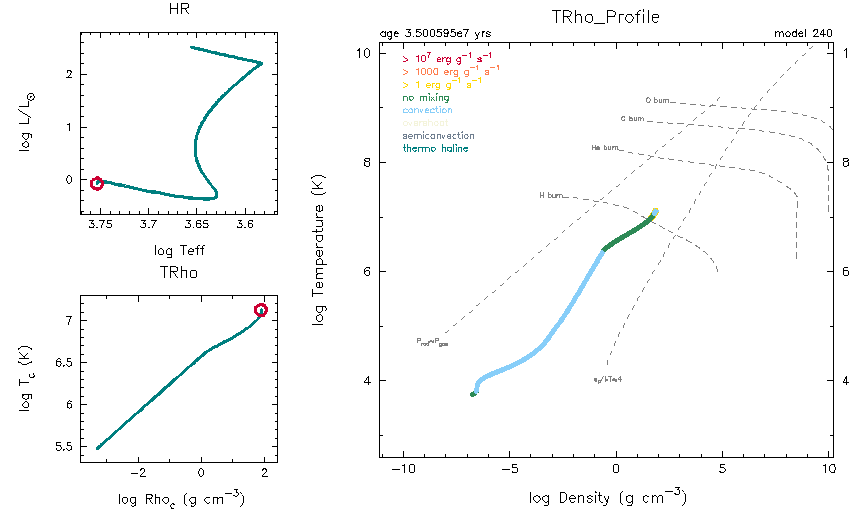
\includegraphics[width=0.9\textwidth]{Grid1_00240}
\caption{Graphical output from a \mesa\ run of a $\val{1}{\Msun}$ PMS star. \label{f.mesa-fig}}
\end{figure}

The large plot labeled `|TRho_profile|' shows the run of temperature $T$ versus density $\rho$ in the star, with the various colors indicating mixing and energy generating regions. The small plot labeled `|HR|' traces the history of luminosity $L$, in units of the solar luminosity $\Lsun$, versus effective temperature $\Teff$. The other small plot labeled `|TRho|' traces the history of the central temperature $T_{c}$ versus the central density $\rho_{c}$.

\begin{exercisebox}[Contraction of a star to the main sequence]
\begin{enumerate}
\item How long did the star take to contract to the main sequence?
\item What are $L$, $\Teff$, $T_{c}$, and $\rho_{c}$ when the star begins H burning?
\item Describe how the fraction of the star that is convective changes during the run.
\end{enumerate}
\end{exercisebox}

\subsection{A peak under the hood}
To understand what just happened, we start with the command `|./rn|'. This is just a script---you can open it with a text editor---containing the following.
\VerbatimInput{introduction/1M-pms/rn}
This just gets some information about the version of \mesa\ being used (the `|svn info|' directive), removes any pre-existing file with restart information, prints the date, runs star, and then prints the date again.

The command `|star|' is built from the source code in `|src/run.f|'. This is a very short program.  The relevant lines
\VerbatimInput[firstline=11,lastline=16]{introduction/1M-pms/src/run.f}
direct the program to read in parameters from a file `|inlist|' and then hand control to a subroutine, `|do_run_star|', within the \mesa\ library.

The file `|inlist|', is divided into three sections (each section begins with an `|&|' followed by the section name and ends with a `|/|'): `|star_job|', `|controls|', and `|pgstar|'.  The bang `|!|' denotes the start of a comment. This list is rather simple. The first section
\VerbatimInput[firstline=1,lastline=9]{introduction/1M-pms/inlist}
tells \mesa\ to read another file, `|1M_pms.inlist|'. The second section, `|&controls|' also tells \mesa\ to read in `|1M_pms.inlist|'. It is in `|1M_pms.inlist|' that all of the settings are placed, so take a quick peek at that file.  For example, in section `|&star_job|' the lines
\VerbatimInput[firstline=21,lastline=22]{introduction/1M-pms/1M_pms.inlist}
tell \mesa\ to pause and wait for the user to hit `|return|' before ending the code, and to activate the plotting windows. In section `|&controls|' the lines
\VerbatimInput[firstline=31,lastline=32]{introduction/1M-pms/1M_pms.inlist}
tell \mesa\ the initial mass and metallicity of the star, while the lines
\VerbatimInput[firstline=42,lastline=43]{introduction/1M-pms/1M_pms.inlist}
tell \mesa\ to stop when the total power from nuclear burning, $L_{\mathrm{nuc}}$, exceeds $0.95 L$, where $L$ is the total surface luminosity.

The third section of `|inlist|'
\VerbatimInput[firstline=18,lastline=26]{introduction/1M-pms/inlist}
reads in the parameters for the plot from `|basic_plot.inlist|'. There is another parameter file, `|track_scaled_vars.inlist|', but the flag to read that file is 
`|read_extra_pgstar_inlist2 = .false.|'  As you might guess, you'll be using this later on in the assignment.

\begin{center}
\fbox{\parbox{0.96\textwidth}{\textbf{Question:} There is a reason for nesting the parameter inlist files. Can you discern what that reason is?}}
\end{center}

Now that you've seen how the code in action, we are going to look a bit more at the architecture of \mesa. If you do `|ls $MESA_DIR|', you will see that \mesa\ is divided into modules: `|eos|' computes the equation of state, `|kap|' computes the opacity, and so forth. Within each module are two folders, `|public|' and `|private|'.  The `|public|' folder contains the interface of that module. The source file ending with `|_def.f|' contains the data structures used by that module, and the source file ending with `|_lib.f|' contains the routines for that module. The |private| directory contains the inner machinery of the module.

All of these modules can be used by themselves; the `|star|' module puts everything together to simulate stellar evolution. What |star| does is to evolve a stellar model---a complete description of a star at a given instant of time---forward in time by some amount $\Delta t$. String together a sequence of such models and you have a representation of the star's evolution. These models are not evenly spaced in time; rather, \mesa\ adjusts $\Delta t$ to keep the models accurate within specified tolerances. The |star| module contains, in addition to the |public| interface and |private| machinery, additional routines in the folder |job| for starting a run from some initial model and stopping that run when a specified condition is met.

\subsection{A MESA project}

The \mesa\ code that you installed is a library, a collection of routines that when combined simulate the evolution of a stellar-like object. To put everything together, you create a directory, such as `|1M-pms|'.  A template for such a directory is contained in `|$MESA_DIR/star/work|'---consult the `|README|' file there for instructions. 

The working directory is organized into several sub-directories. The `|make|' folder contains the `|makefile|' script for compiling the code. The `|src|' folder contains, in addition to the top-level `|run.f|' code, a collection of customizable routines in the file `|run_star_extras.f|'. In addition to these folders, the working directory contains a set of inlist files; these, as mentioned above, contain all of the parameters necessary to control the \mesa\ run and its output.  The complete listings of parameters and their default settings are contained in the directory `|$MESA_DIR/star/defaults|' in the three files `|*.defaults|'. The inlists in the work directory only need to contain those parameters that differ from the defaults.

The final components of the working directory are sub-directories to hold the output of \mesa.  The names of these are customizable and can be set in the inlists; by default, the main two are called `|LOGS|' and `|photos|'.  Within `|LOGS|' are the file `|history.data|' and the files `|profile|\textit{dd}|.data|'. The `|history.data|' file contains the time evolution of global stellar properties, such as luminosity, radius, surface effective temperature, and so on. The `|profile|\textit{dd}|.data|' files contain ``snapshots'' of the star's structure: the run of temperature, density, pressure, and so on with location within the star. 

\subsection{Exercise: customizing MESA output}

After that brief overview of the \mesa\ architecture, let's do something concrete: we'll customize \mesa\ to have it generate a plot of a variable that we define.  In this chapter, we've argued that the central pressure of a star should scale as $P_{c}\propto GM^{2}/R^{4}$. We also found that the central density should scale as the mean density, $\rho_{c}\propto \bar{\rho} = 3M/(4\pi R^{3})$. Exercise~\ref{ex.central-temperature} asks you to find the central temperature in terms of $M$, $R$, and mean molecular weight $\mu$. What the derivation in the chapter doesn't tell us is the coefficient $\rho_{c}/\bar{\rho}$ and its counterparts for pressure and temperature.  We can use \mesa, however, to test these scalings and extract these constants of proportionality.

To do this, we modify the code in `|src/run_star_extras.f|'.  What we want is for \mesa\ to calculate $P_{\mathrm{scale}} = GM^{2}/R^{4}$, $\rho_{\mathrm{scale}} = \bar{\rho}$, and $T_{\mathrm{scale}}$, and then write out the values of $P_{c}/P_{\mathrm{scale}}$, $\rho_{c}/\rho_{\mathrm{scale}}$, and $T_{c}/T_{\mathrm{scale}}$ in the file `|history.data|'. To do this, we first tell \mesa\ how many extra columns in `|history.data|' we need:
\VerbatimInput[firstline=96,lastline=104,gobble=8]{introduction/1M-pms/src/run_star_extras.f}
Here I am adding one column, which will be $P_{c}/P_{\mathrm{scale}}$.  When you implement the other scalings, you'll change the variable \verb|how_many_extra_history_columns| to reflect that we need three columns.

Next, we need to compute the data for these columns.  We therefore modify the following routine.
\VerbatimInput[firstline=107,lastline=154,gobble=8]{introduction/1M-pms/src/run_star_extras.f}
In detail, we first declare the extra variables we need.
\VerbatimInput[firstline=113,lastline=113,gobble=8]{introduction/1M-pms/src/run_star_extras.f}
Next, we give each column a name.
\VerbatimInput[firstline=124,lastline=126,gobble=8]{introduction/1M-pms/src/run_star_extras.f}
Notice that the latter two are commented out (`|!|'); for this example; you'll need to uncomment them to print out the other variables.

We are then ready to compute our values.  Note that \mesa\ defines many physical constants in `|$MESA_DIR/const/public/const_def.f|'; we therefore use this in line 130 for $G$, and you can read the hint in lines 143ff. Next, we need to get the values of $M$, $R$, $\mu_{c}$, $P_{c}$, $\rho_{c}$, and $T_{c}$. These are provided in a data structure |s|, which the routine fetches
\VerbatimInput[firstline=116,lastline=116,gobble=8]{introduction/1M-pms/src/run_star_extras.f}
from the variable |id| that is passed to the routine.  To see a complete list of what is in this data structure, look at `|$MESA_DIR/star/public/star_data.inc|'. I've already taken care of computing $M$, $R$, $\mu_{c}$, and $P_{\mathrm{scale}}$ for you.  The values of our scaled variables are then stored in the array `|vals|'; you will fill in the second and third members of the array.

If you look in `|LOGS/history.data|', you should see that the last column is indeed `|Pc_scaled|', as expected. Of course, we'd like to display it graphically, and \mesa\ does predefine plots that can display values in `|history.data|'. We customized the output in `|track_scaled_vars.inlist|':
\VerbatimInput{introduction/1M-pms/track_scaled_vars.inlist}
To use this, we activate the window by setting the flag in line 3 to `|.true.|'. If we want to save our output, we set the `|file_flag = .true.|' in line 11.  

\UndefineShortVerb{\|}

